\documentclass[11pt]{exam}

\usepackage{amsmath}
\usepackage{graphicx}
\usepackage{geometry}
\usepackage{etoolbox}
\BeforeBeginEnvironment{choices}{\par\nopagebreak\minipage{\linewidth}}
\AfterEndEnvironment{choices}{\endminipage}
\geometry{
a4paper,
total={185mm,257mm},
left=10mm,
top=25mm,
bottom=10mm
}

\begin{document}
\setlength{\voffset}{-0.5in}
\setlength{\headsep}{5pt}

\fbox{\fbox{\parbox{8cm}{\centering
\vspace{2mm}
Testat - Versuch J - Ultraschall - 3
\vspace{2mm}
}}}
\hspace{2mm}
\makebox[0.25\textwidth]{Name:\enspace\hrulefill} \hspace{5mm}
\makebox[0.2\textwidth]{Datum:\enspace\hrulefill}
\vspace{4mm}

\begin{questions}

\question Wie hoch ist die Frequenz des in der Graphik dargestellten Signals? 

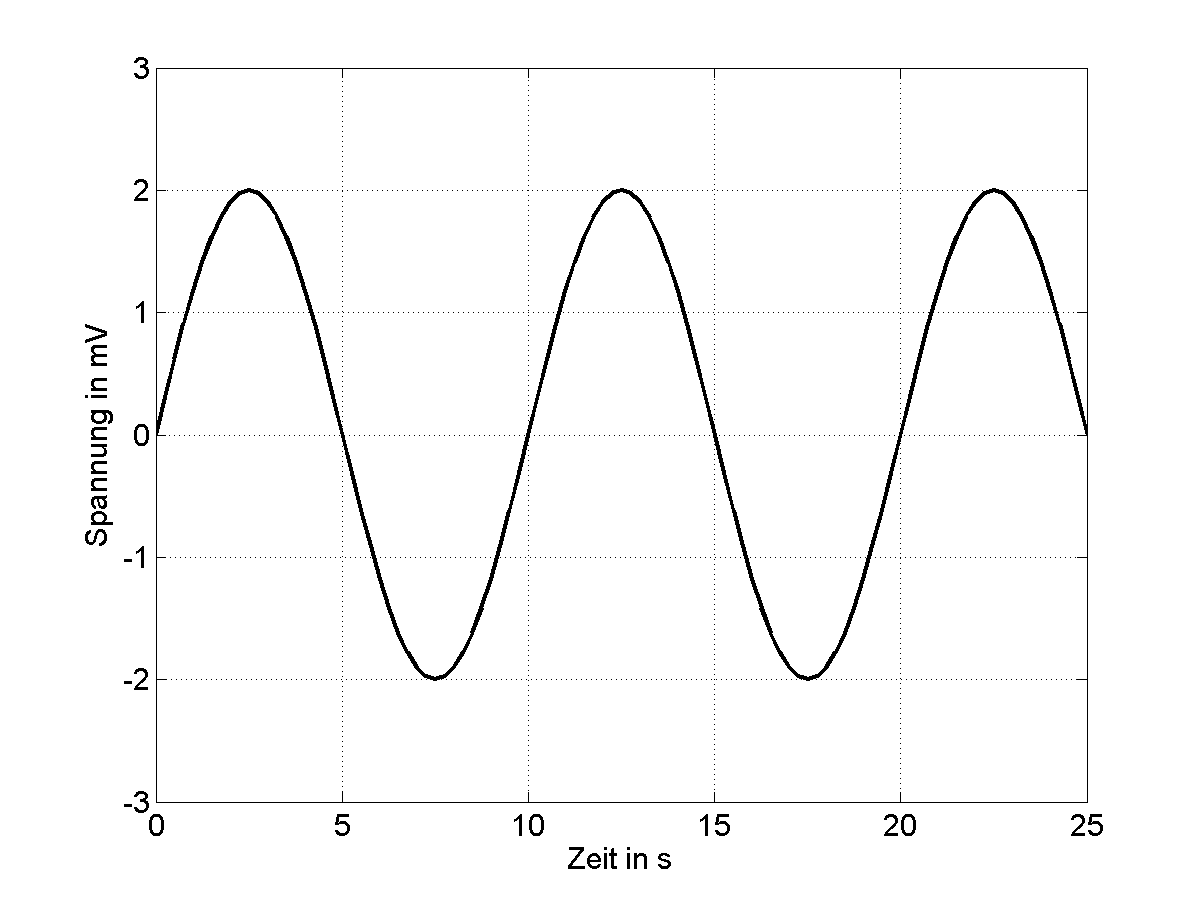
\includegraphics[width=0.5\textwidth]{../../../questions/J/images/SchallSinus1.png}

\begin{choices}
	\choice 5 s
	\choice 0,2 Hz
	\choice 10 s
	\choice 0,1 Hz (correct)
	\choice 10 Hz
\end{choices}

\vspace{3mm}\question Welche der folgenden Formeln für die Schallgeschwindigkeit ist richtig?( \( c \) Schallgeschwindigkeit, \(T \) Periodendauer, \( f \) Frequenz, \( \lambda \) Wellenlänge)

\begin{choices}
	\choice \( c=T \cdot \lambda \)
	\choice \( c=f \cdot \lambda \) (correct)
	\choice \( c=T \cdot f \)
	\choice \( c=\frac{T}{\lambda} \)
	\choice \( c=\frac{f}{\lambda} \)
\end{choices}

\vspace{3mm}\question Mit einem Echolot soll eine Position eines Gegenstandes in einem Medium mit einer Schallgeschwindigkeit von 1000 m/s überprüft werden. Dazu wird durch eine Sonde eine Schallwelle ausgestrahlt, die an dem Gegenstand reflektiert wird und daraufhin wieder an der Sonde eintrifft. Es dauert 10 s, bis die Schallwelle nach ihrer Aussendung wieder an der Sonde eintrifft. Wie weit liegt der Gegenstand von der Sonde entfernt?

\begin{choices}
	\choice etwa 500 m
	\choice etwa 5000 m (correct)
	\choice etwa 10000 m
	\choice etwa 100 m
	\choice etwa 20000 m
\end{choices}

\vspace{3mm}\question Auf welchem Effekt beruht die Erzeugung und Messung von Ultraschallwellen mittels eines Kristalls?

\begin{choices}
	\choice Piezoeffekt (correct)
	\choice Hall-Effekt
	\choice Comptoneffekt
	\choice Faradayeffekt
	\choice Fotoeffekt
\end{choices}

\vspace{3mm}\question Zwei Schallwellen breiten sich gleichzeitig in unterschiedlichen Medien aus. Welche Aussage ist richtig?

\begin{choices}
	\choice Wenn beide Wellen die gleiche Periodendauer haben, dann haben sie auch die gleiche Wellenlänge.
	\choice Wenn beide Wellen die gleiche Frequenz haben, dann haben sie auch die gleiche Schallgeschwindigkeit. (correct)
	\choice Wenn beide Wellen die gleiche Frequenz haben, dann haben sie auch die gleiche Periodendauer.
	\choice Wenn beide Wellen die gleiche Frequenz haben, dann haben sie auch die gleiche Wellenlänge.
	\choice Wenn beide Wellen die gleiche Wellenlänge haben, dann haben sie auch die gleiche Schallgeschwindigkeit.
\end{choices}

\vspace{3mm}\end{questions}

\end{document}
